\documentclass{beamer}

\usepackage[british]{babel}
\usepackage{graphicx,hyperref,ru,url}

\title[AI@Webscale Presentation]{
  AI at the Webscale Project Results}

\author[Bas Bootsma, Fenno Vermeij]{Bas Bootsma \& Fenno Vermeij}

\institute[Radboud University Nijmegen]{Radboud University Nijmegen}

\date{\today}

\begin{document}

\begin{frame}
  \titlepage
\end{frame}

\begin{frame}
	\frametitle{Approach}	
	\begin{itemize}
		\item Epsilon-greedy
		\item Gibbs-sampling
		\item Thompson-sampling
	\end{itemize}
\end{frame}

\begin{frame}
	\frametitle{Model}
	
		\begin{align*} r = \beta_0 + \beta_{x_1} c_1 + &\ldots + \beta_{x_k} c_k + \\
	    \beta_{y_1} a_1 + &\ldots + \beta_{y_l} a_l + \\
	    \beta_{z_1} c_1a_1 + &\ldots + \beta_{z_m} c_ka_l 
	    \end{align*}
	    \begin{itemize}
		\item Reward for update: use price $\cdot$ effect instead of effect
	\end{itemize}
\end{frame}

\begin{frame}
	\frametitle{Visualization}
	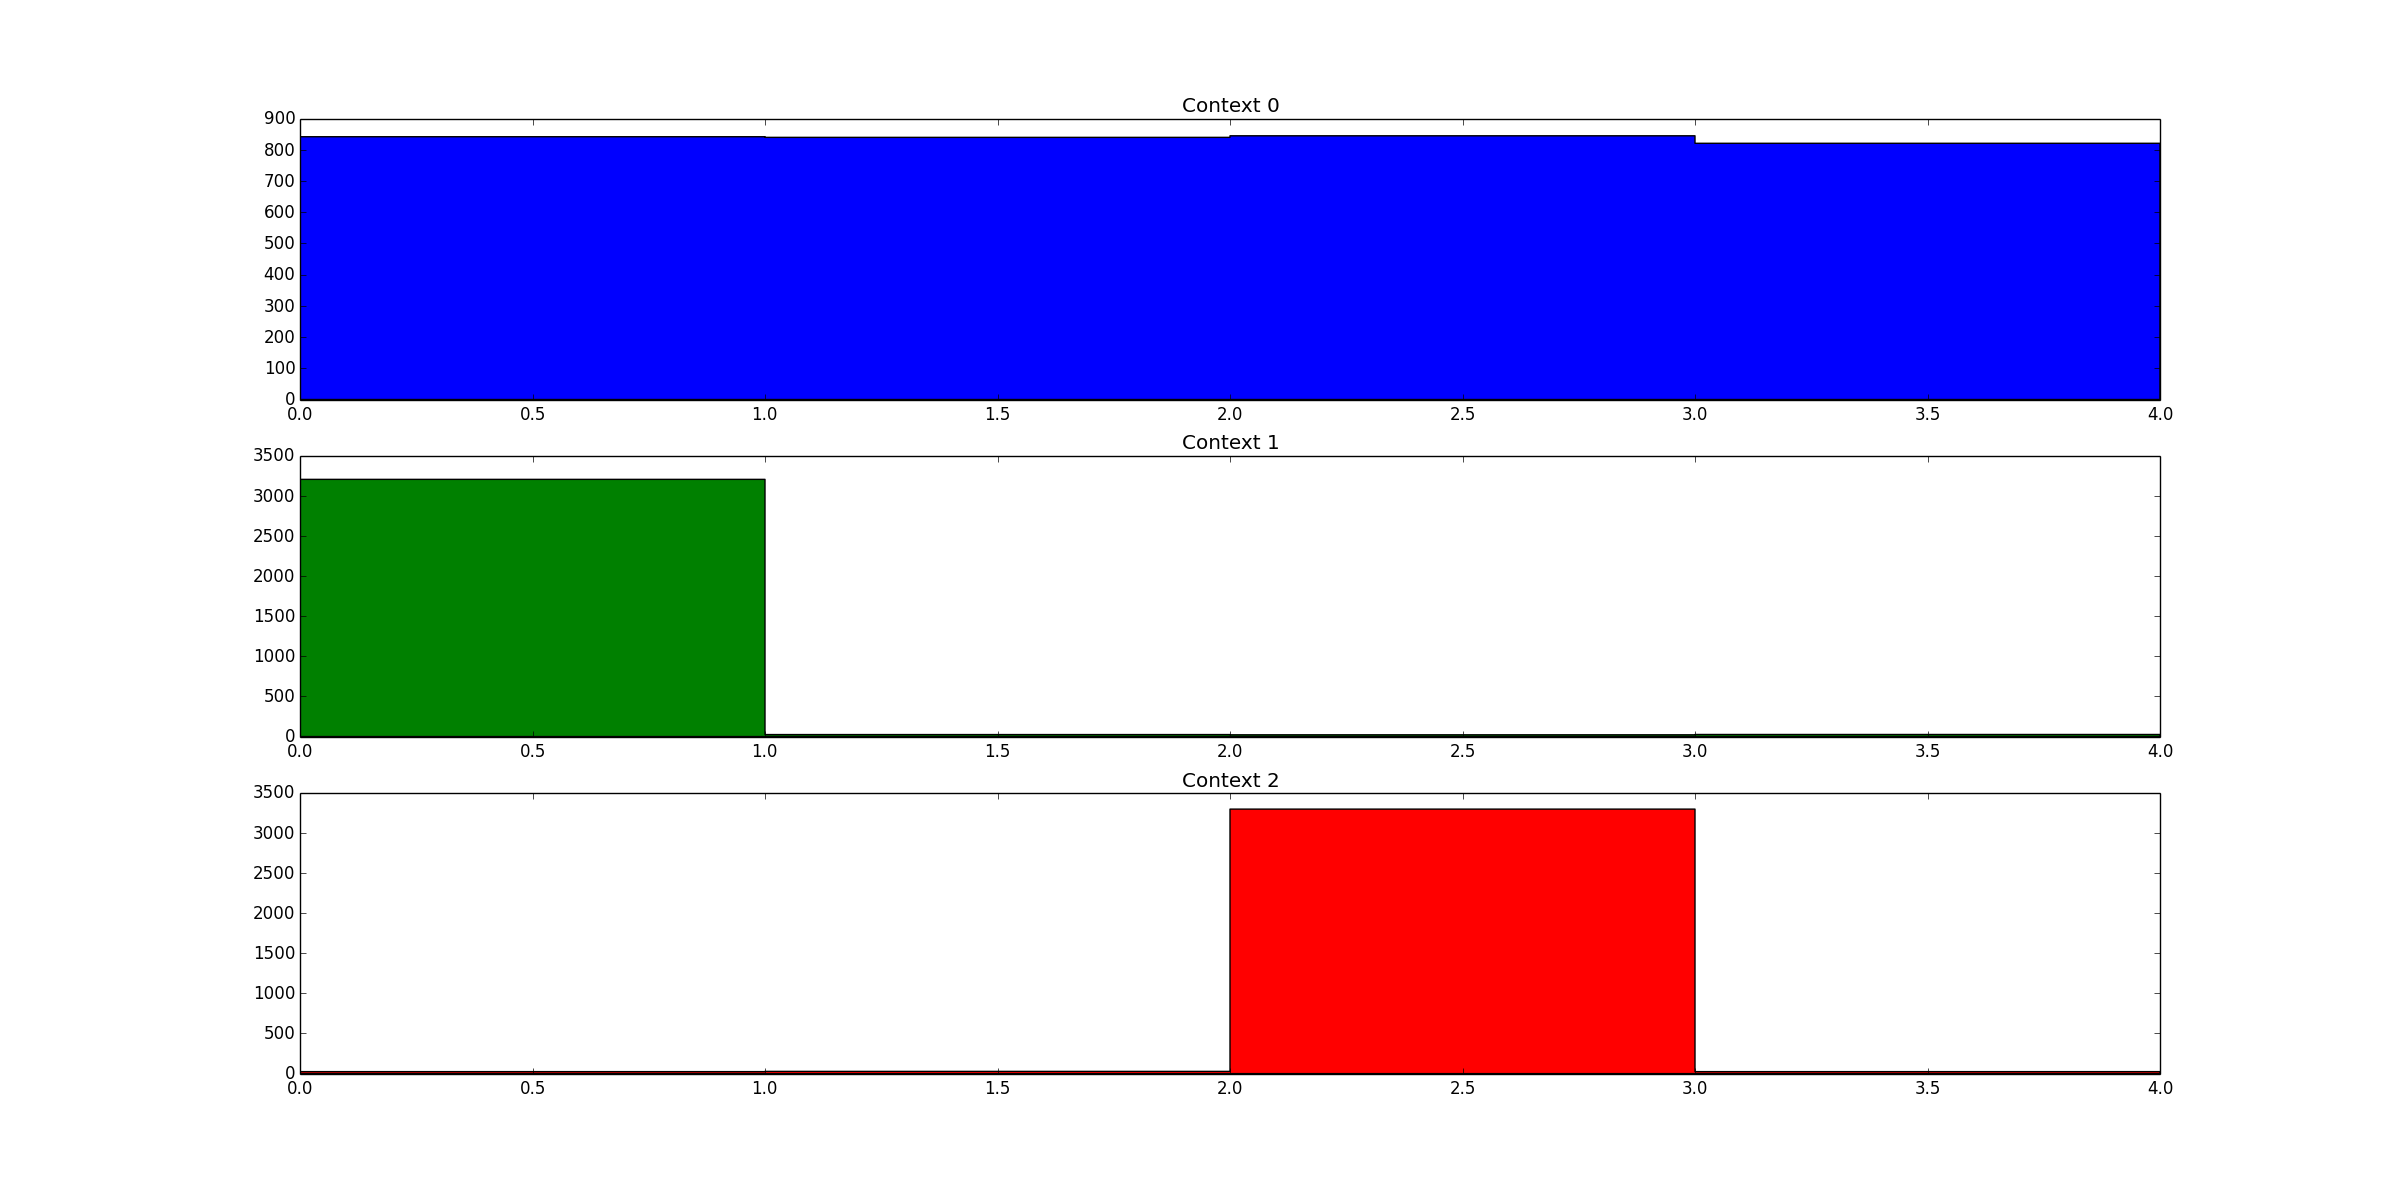
\includegraphics[width=\textwidth]{test.png}
\end{frame}

\begin{frame}
	\frametitle{Visualization}
	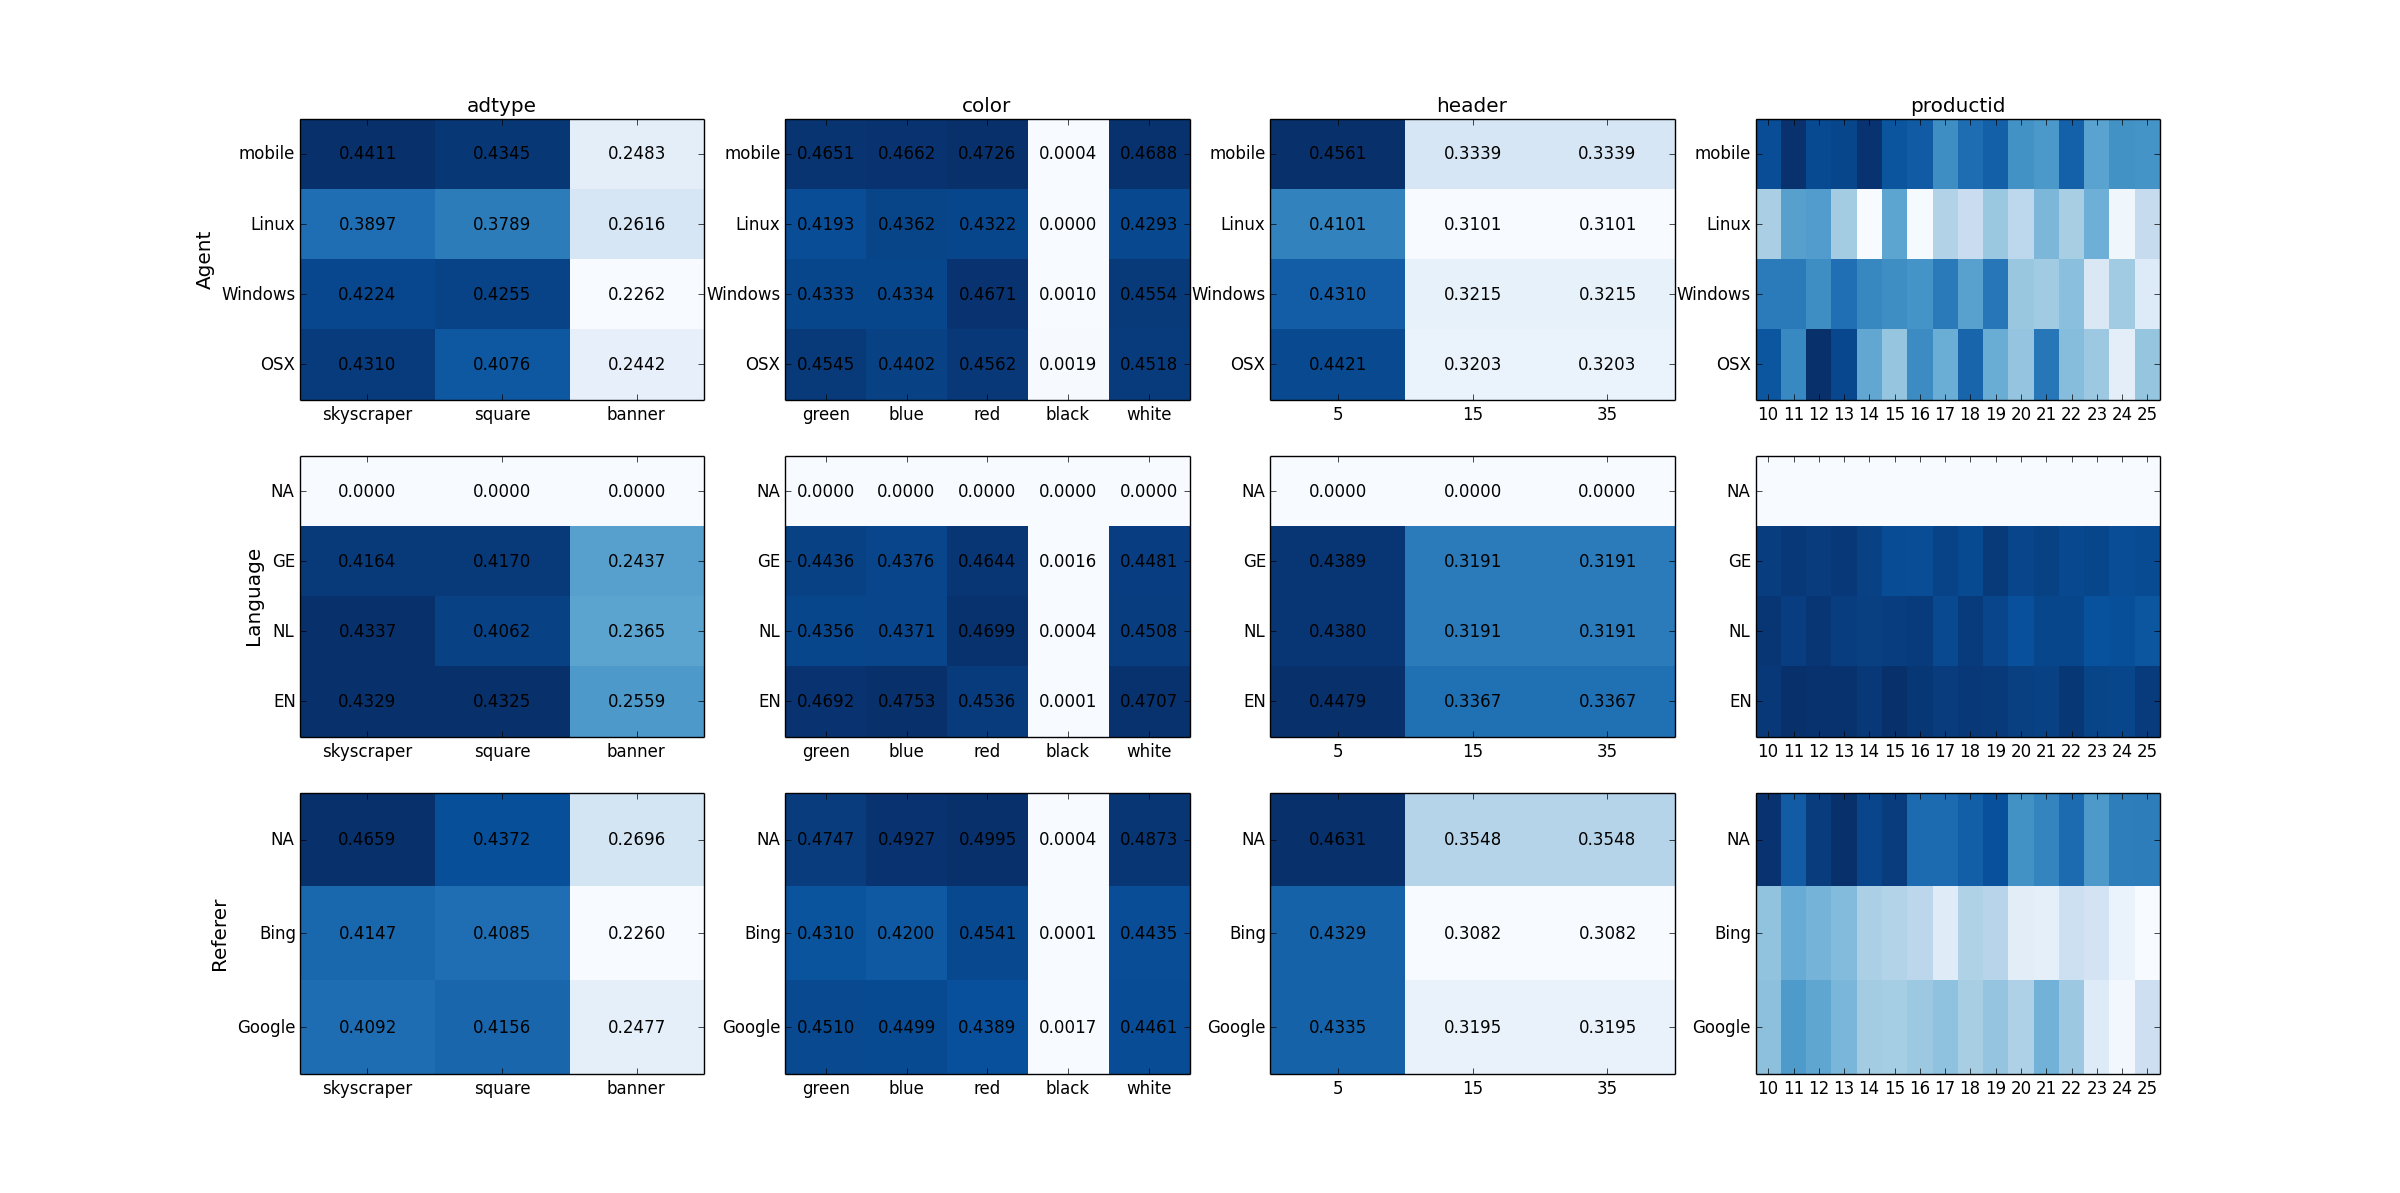
\includegraphics[width=\textwidth]{viewer.png}
\end{frame}


\begin{frame}
	\frametitle{Misc. Improvements}
	\begin{itemize}
		\item Price: Maximize polynomial: $\beta_0 + \beta_1 \cdot p + \beta_2 \cdot p^2$ %in buckets: [1, 5, 10, 15, 20, 25, 30, 35, 40, 45, 50]
		\item Multivariate Gaussian speedup: use Cholesky transformation
		\item Predict 5000 random pages to give model `warm start' before doing actual predictions.
		\item Userid: add extra features: average price user paid previously, if user has bought anything previously
	\end{itemize}
\end{frame}


\begin{frame}
  \frametitle{Results}

  \begin{itemize}
    \item Average reward: 20.0605
    \item Standard deviation: 24.507
    \item Time taken: 1:25 per runId
    \item Any questions?
  \end{itemize}
\end{frame}

\end{document}
